\documentclass[../../main.tex]{subfiles}

\begin{document}
\section{Tensor Networks}
    Our goal now is to focus on a subclass of models over $\Sigma^*$. To this end, we analyze \emph{tensor networks}.

    \bigskip
    We denote a tensor \( T_v \) with \( k \) axes of sizes \( D_v = \{d_1, \dots, d_k\} \) as a function
    \[
    T_v : [d_1] \times \dots \times [d_k] \to \mathbb{R}_{\geq 0}.
    \]
    As a shorthand, we write
    \[
        [D_v] \coloneqq [d_1] \times \dots \times [d_k] \quad .
    \]
    Since indexing is usually clear from context, we treat \( D_v \) as a multiset of axis sizes.

    Given two tensors \( T_u \) and \( T_v \) that share a common axis of size \( d_e \), their contraction over this axis produces a new tensor \( T_C \) with dimension set
    \[
    D_C = (D_u \setminus \{d_e\}) \cup (D_v \setminus \{d_e\}) \quad ,
    \]
    defined as
    \[
    T_C(i) = \sum_{i_e \in [d_e]} T_u(i_{D_u}, i_{e}) \cdot T_v(i_{D_v}, i_{e}) \quad ,
    \]
    where \( i \in [D_C] \). Note that $d_e \not \in D_C$, which is why we explicitly included index $i_{e}$ in the summation.

    \begin{definition}[Tensor Network over \( \Sigma^n \)]
    A \emph{tensor network} \( \mathcal{T} \) over \( \Sigma^n \) is defined by a graph \( G = (V, E) \) with the following structure:
    \begin{itemize}
        \item \( V \) is the set of vertices, where each vertex \( v = (\text{layer}, \text{index}) \in V \) corresponds to a tensor \( T_v \) with axis sizes \( D_v = \{d_1, \dots, d_k\} \). Let \( V_{\text{layer}} \subseteq V \) denote the set of all vertices at a given layer.
        
        \item The input set \( I = (T_{0,1}, \dots, T_{0,n}) \subset V \) consists of tensors each having a single axis of size \( |\Sigma| \). These serve as the one-hot-encoded inputs corresponding to a string \( w \in \Sigma^n \).
        
        \item \( E \subseteq \{\{u, v\} \mid u \in V_l,\, v \in V_{l+1}\} \) is the set of edges. Each edge \( e = \{u, v\} \) represents a shared index of size \( d_e \) between tensors \( T_u \) and \( T_v \), which is summed over during contraction.
        
        \item The usual tensor network constrains: For each vertex \( v \in V \), the degree \( \deg(v) \) must match the number of axes \( |D_v| \), and shared indices must correspond to same axis sizes.
    \end{itemize}

    Once the input tensors are initialized with one-hot encodings derived from a string \( w \in \Sigma^n \), the network computes a scalar output \( \mathcal{T}(w) \). This induces a probability distribution over \( \Sigma^n \) defined by:
    \[
    S_{n, \mathcal{T}}(w) \coloneqq \frac{\mathcal{T}(w)}{\sum_{w' \in \Sigma^n} \mathcal{T}(w')}.
    \]
    \end{definition}

    \begin{figure}[h]
    \center
    \begin{tikzpicture}[
        node distance=1.8cm and 2.5cm,
        every node/.style={draw, circle, minimum size=1.2cm}
    ]

    % Layer 0 (Input) at the bottom
    \node (i1) at (0, 0) {$T_{0,1}$};
    \node (i2) [right=of i1] {$T_{0,2}$};
    \node (i3) [right=of i2] {$T_{0,3}$};

    % Layer 1 (Hidden) in the middle
    \node (h1) [above=of i1] {$T_{1,1}$};
    \node (h2) [above=of i2] {$T_{1,2}$};
    \node (h3) [above=of i3] {$T_{1,3}$};

    % Layer 2 (Output) at the top
    \node (o1) [above=of h2] {$T_{2,1}$};

    % Edges: Input to Hidden
    \draw (i1) -- (h1);
    \draw (i2) -- (h2);
    \draw (i3) -- (h3);

    % Edges: Hidden to Output
    \draw (h1) -- (o1);
    \draw (h2) -- (o1);
    \draw (h3) -- (o1);

    % Layer labels
    \node[draw=none, below=0.2cm of i2] {Input Layer};
    \end{tikzpicture}
    \caption{A basic tensor network over $\Sigma^3$.}
    \end{figure}


    \bigskip
    \begin{definition}[Normalization of Tensor Networks]
        Let $\mathcal{T}$ be a tensor network over $\Sigma^n$ with scalar output $\mathcal{T}(w)$ for each $w \in \Sigma^n$. Define the total mass of the network as
        \[
            |\mathcal{T}| \coloneqq \sum_{w \in \Sigma^n} \mathcal{T}(w) \quad .
        \]
        We say $\mathcal{T}$ is \emph{normalized} iff $|\mathcal{T}| = 1$.

        Let $H \coloneqq V \setminus I$ be the set of non-input tensors, and define $|H|$ as its cardinality. The \emph{induced normalized tensor network} $\dfrac{\mathcal{T}}{|\mathcal{T}|}$ is the same network as $\mathcal{T}$, but each entry of each tensor in $H$ is scaled by the factor $\dfrac{1}{\sqrt[|H|]{|\mathcal{T}|}}$.
    \end{definition}


    \begin{lemma}
        Let $J \subseteq [n]$ and let $\mathcal{T}$ be a tensor network over $\Sigma^n$. Define a modified network $\mathcal{T}_J$ where for all $j \in J$, the input tensor $T_{0,j}$ is initialized to the all-ones vector (i.e., $\mathbf{1} \in \mathbb{R}^{|\Sigma|}$). Then for any $w \in \Sigma^{[n] \setminus J}$:
        \[
            \sum_{w_J \in \Sigma^{|J|}} \mathcal{T}(w_J, w) = \mathcal{T}_J(w) \quad .
        \]
    \end{lemma}
    \begin{proof}
    The tensor network $\mathcal{T}(w)$ evaluates to a scalar obtained by contracting the network, where each input tensor $T_{0,j}$ is initialized with a one-hot vector corresponding to the symbol $w_j \in \Sigma$.

    For $j \in J$, replacing the one-hot vector by the all-ones vector is equivalent to summing over all possible $w_j \in \Sigma$. That is, for fixed $w \in \Sigma^{[n] \setminus J}$,
    \[
        \mathcal{T}_J(w) = \sum_{w_J \in \Sigma^{|J|}} \mathcal{T}(w_J, w) \quad ,
    \]
    since the multilinearity of the network ensures that the contraction distributes over summation in each input.

    Formally, each contraction involving an input tensor $T_{0,j}$ with the one-hot vector $\delta_{w_j}$ is replaced by a sum over $\delta_{w_j}$ for all $w_j \in \Sigma$, i.e., the all-ones vector $\mathbf{1}$. The result of the total contraction is thus the sum over all \( w_J \in \Sigma^{|J|} \) of \( \mathcal{T}(w_J, w) \), as required.
    \end{proof}

    \begin{corollary}
        Let $\mathcal{T}$ be a tensor network over $\Sigma^n$, and let $\mathcal{T}_{[n]}$ be the network where all input tensors are initialized to the all-ones vector. Then:
        \[
            \mathcal{T} \text{ is normalized} \iff \mathcal{T}_{[n]} = 1 \quad ,
        \]
        i.e., the total contraction of the network with all-one input tensors equals 1.
    \end{corollary}

    \begin{lemma}
        Let $\mathcal{T}$ be a tensor network over $\Sigma^n$. The induced normalized tensor network $\frac{\mathcal{T}}{|\mathcal{T}|}$ is indeed normalized and we have for all $w \in \Sigma^n$:
        \[
            S_{n, \mathcal{T}}(w) = S_{n, \frac{\mathcal{T}}{|\mathcal{T}|}}(w) \quad .
        \]
    \end{lemma}
    \begin{proof}
        Let $H$ be the set of non-input tensors in $\mathcal{T}$, and let $|H| = m$. In the induced normalized network, every tensor in $H$ is scaled by a factor $\alpha = \dfrac{1}{\sqrt[m]{|\mathcal{T}|}}$. Since the final output $\mathcal{T}(w)$ is a multilinear contraction over the tensors, this means the scalar output for any $w \in \Sigma^n$ becomes:
        \[
            \left( \prod_{v \in H} \alpha \right) \cdot \mathcal{T}(w) = \alpha^m \cdot \mathcal{T}(w) = \frac{1}{|\mathcal{T}|} \cdot \mathcal{T}(w) \quad .
        \]
        Hence,
        \[
            \left(\frac{\mathcal{T}}{|\mathcal{T}|}\right)(w) = \frac{\mathcal{T}(w)}{|\mathcal{T}|} \quad .
        \]

        Summing over all \( w \in \Sigma^n \),
        \[
            \left| \frac{\mathcal{T}}{|\mathcal{T}|} \right| = \sum_{w \in \Sigma^n} \frac{\mathcal{T}(w)}{|\mathcal{T}|} = \frac{1}{|\mathcal{T}|} \sum_{w \in \Sigma^n} \mathcal{T}(w) = \frac{|\mathcal{T}|}{|\mathcal{T}|} = 1 \quad .
        \]

        Moreover, since the normalization rescales all outputs by the same constant, the softmax remains unchanged:
        \[
            S_{n, \frac{\mathcal{T}}{|\mathcal{T}|}}(w) = \frac{\left( \frac{\mathcal{T}(w)}{|\mathcal{T}|} \right)}{\sum_{w' \in \Sigma^n} \left( \frac{\mathcal{T}(w')}{|\mathcal{T}|} \right)} = \frac{\mathcal{T}(w)}{|\mathcal{T}|} \cdot \frac{1}{1} = S_{n, \mathcal{T}}(w) \quad .
        \]

        This completes the proof.
    \end{proof}



    One might ask whether our definition for tensor networks is bit restrictive, as it only allows for contraction over \emph{pairs} of tensors. But what if we wanted to contract, say, three tensors at once over a common index?

    \begin{proposition}
        Let $V' \subseteq V$ be a set of tensors in a tensor network, each containing an axis of dimension $d$ labeled by a shared index $i$. Contracting all tensors in $V'$ over the shared index $i$ is equivalent to contracting each tensor individually with a single tensor 
        \[
        \delta_{|V'|} : [d]^{|V'|} \mapsto \mathbb{R}_{\geq 0}
        \]
        defined by
        \[
        \delta_{|V'|}(i_1, \dots, i_{|V'|}) = 
        \begin{cases}
        1 & \text{if } i_1 = \dots = i_{|V'|} \ , \\
        0 & \text{otherwise.}
        \end{cases}
        \quad .
        \]
        That is, a full contraction over a shared index can be implemented by introducing a single copy tensor connected to each tensor in $V'$.
    \end{proposition}

\begin{proof}
Each tensor $T_v$ for $v \in V'$ has an index \( i \in [d] \) corresponding to the shared axis. The contraction over this index is defined by summing over the common value of \( i \) across all tensors:
\[
\sum_{i=1}^d \prod_{v \in V'} T_v(\dots, i, \dots) \quad .
\]

Now consider a new tensor \( \delta_{|V'|} \) of order \( |V'| \), defined as 1 if all indices are equal and 0 otherwise. Let each tensor \( T_v \) maintain its original indices, but connect to \( \delta_{|V'|} \) via the position corresponding to \( v \).

The contraction over this shared structure gives:
\[
\sum_{i_1, \dots, i_{|V'|}} \left( \prod_{v \in V'} T_v(\dots, i_v, \dots) \right) \delta_{|V'|}(i_1, \dots, i_{|V'|}) \quad .
\]

By definition of \( \delta_{|V'|} \), this enforces \( i_1 = \dots = i_{|V'|} \), reducing the above to:
\[
\sum_{i=1}^d \prod_{v \in V'} T_v(\dots, i, \dots) \quad ,
\]
which is exactly the original contraction. Hence, the two constructions are equivalent.
\end{proof}

    \begin{figure}[h]
        \center
        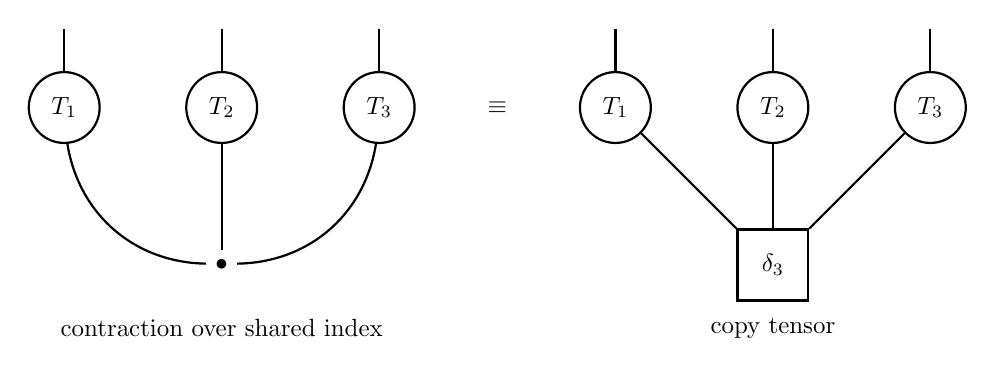
\begin{tikzpicture}[thick, scale=1.0, every node/.style={scale=0.9}]
            % Left side - shared index (hyperedge)
            \node[draw, circle, minimum size=1cm] (L1) at (-4, 0) {$T_1$};
            \node[draw, circle, minimum size=1cm] (L2) at (-2, 0) {$T_2$};
            \node[draw, circle, minimum size=1cm] (L3) at (0, 0) {$T_3$};
            \node (H) at (-2, -2) {$\bullet$};
            \node at (-2, -2.8) {contraction over shared index};

            % Curved edges to show shared index
            \draw[bend right=40] (L1) to (H);
            \draw (L2) to (H);
            \draw[bend left=40] (L3) to (H);


            \node at (1.5, 0) {$\equiv$};

            % Right side - copy tensor
            \node[draw, circle, minimum size=1cm] (R1) at (3, 0) {$T_1$};
            \node[draw, circle, minimum size=1cm] (R2) at (5, 0) {$T_2$};
            \node[draw, circle, minimum size=1cm] (R3) at (7, 0) {$T_3$};

            \node[draw, rectangle, minimum size=1cm, inner sep=0pt] (delta) at (5, -2) {$\delta_3$};

            % Connections to copy tensor
            \draw[-] (delta) -- (R1);
            \draw[-] (delta) -- (R2);
            \draw[-] (delta) -- (R3);

            \node at (5, -2.8) {copy tensor};

            % Optional: inputs
            \draw[-] (L1) -- (-4, 1);
            \draw[-] (L2) -- (-2, 1);
            \draw[-] (L3) -- (0, 1);
            \draw[-] (R1) -- (3, 1);
            \draw[-] (R2) -- (5, 1);
            \draw[-] (R3) -- (7, 1);
        \end{tikzpicture}
        \caption{Contracting multiple tensors over one shared index is equivalent to contracting them individually with a single copy tensor.}
    \end{figure}

\subsection{Bulk Marginal Property}
    We are interested in tensor networks that have the bulk marginal property. When further specifying our network structure, we might have a model space for varying word lengths $n$, but not for every $n \in \mathbb{N}$. Take for example the model space of binary trees as shown in figure~\ref{fig:binary_tree_tensor_network}.

    \begin{figure}[h]
        \center
        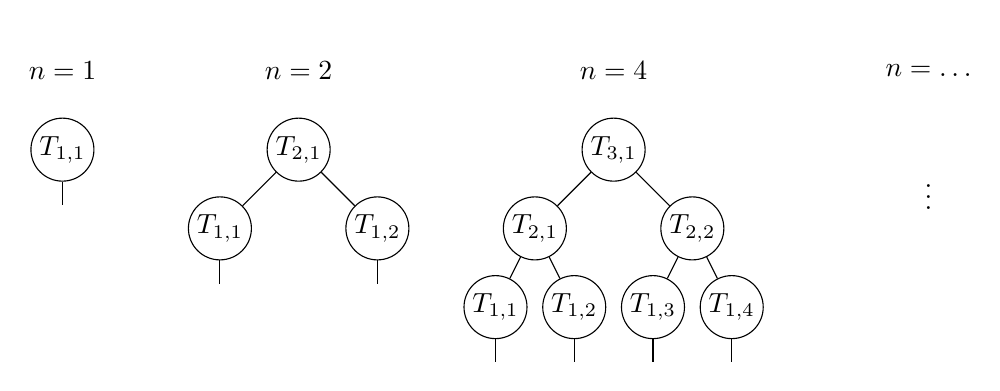
\begin{tikzpicture}[
            every node/.style={circle, draw, minimum size=8mm, inner sep=0pt},
            level distance=10mm,
            sibling distance=10mm,
            edge from parent/.style={draw},
            level 1/.style={sibling distance=20mm},
            level 2/.style={sibling distance=10mm}
        ]

        % Tree with 1 leaf
        \node[draw=none] at (-6,0) {$n=1$};
        \node (t11a) at (-6,-1) {$T_{1,1}$};
        \draw (t11a) -- ++(0,-0.7);

        % Tree with 2 leaves
        \node[draw=none] at (-3,0) {$n=2$};
        \node (t21) at (-3, -1) {$T_{2,1}$} [grow=down]
        child {node (t11b) {$T_{1,1}$}}
        child {node (t12) {$T_{1,2}$}};
        \draw (t11b) -- ++(0,-0.7);
        \draw (t12) -- ++(0,-0.7);

        % Tree with 4 leaves
        \node[draw=none] at (1,0) {$n=4$};
        \node (t31) at (1, -1) {$T_{3,1}$} [grow=down]
        child {node (t21a) {$T_{2,1}$}
            child {node (t11c) {$T_{1,1}$}}
            child {node (t13) {$T_{1,2}$}}}
        child {node (t22) {$T_{2,2}$}
            child {node (t14) {$T_{1,3}$}}
            child {node (t15) {$T_{1,4}$}}};
        \draw (t11c) -- ++(0,-0.7);
        \draw (t13) -- ++(0,-0.7);
        \draw (t14) -- ++(0,-0.7);
        \draw (t15) -- ++(0,-0.7);

        % Dots representing omitted trees
        \node[draw=none] at (5,0) {$n=\dots$};
        \node[draw=none] at (5,-1.5) {$\vdots$};
        \end{tikzpicture}
        \caption{A model space for sequences of length $n = 2^k$.}
        \label{fig:binary_tree_tensor_network}
    \end{figure}

    In definition~\ref{def:induced_bulk_marginal_model} we saw how to construct a model with the desired bulk marginal property based on the base model. However, we might not always have a base model for ever $n \in \mathbb{N}$ like discussed. Luckily, it turns out that this is not an issue, as there are many ways we can build a new model with the bulk marginal property from a base model even if it is only defined on a subset of $\mathbb{N}$. Without a proof, we might do the same procedure as in definition~\ref{def:induced_bulk_marginal_model} but with bigger steps (instead of taking always the consecutive model), and induce the in-between models by marginalizing the bigger ones.

    Alternatively, if we wanted a model with bulk marginal property that itself is also an element of our specified model space, we might ask ourselves, how we can construct a bigger tensor network while preserving the distribution in its leading random variables.
\end{document}